\documentclass[11pt] {article}
\usepackage [utf8] {inputenc}
\title {\textbf{6 Adaptacion del DAO al nuevo modelo relacional}}
\author {Jesús Sánchez Granado}
\usepackage{natbib}
\usepackage{graphicx}
\begin{document}
\maketitle
Tras cambiar la base de datos de mongo por una de SQL, también era necesario hacer la lógica de accesos a la base de datos, por lo que se crearon 4 Data Access Object (DAO a partir de ahora) que se encargarían de las operaciones de cada una de las 4 áreas definidas en el modelo de entidad-relación.

El DAO es un patrón de diseño el trata de proporcionar una interfaz para la comunicación con una base de datos u otro sistema de persistencia de datos. Esta interfaz se encarga de llevar a cabo las operaciones CRUD, es decir creación, lectura, actualización y eliminación de datos y además asegura la independencia entre la lógica de la aplicación y la capa de negocio.

Aunque no eran estrictamente necesarios dado que en javascript no hace falta declarar el tipo de los objetos, se decidió crear objetos transfer para así tener más documentados los campos de cada tipo de objeto.
Un transfer o Data Transfer Object es un objeto cuya única función es guardar la información de cierto objeto y permitir su acceso y manipulación.
De esta forma si hay algún problema, este se detectará cuanto antes y evitará que la aplicación falle repentinamente más avanzada su ejecución.

Los objetos transfer contienen simplemente los atributos deseados de cada tipo de objeto además de las funciones get y set para poder acceder y actualizar la información de dichos atributos.
En conjunto con los DAO, los transfer ayudan aún más a la separación de capas de negocio y lógica.

Los cuatro DAO que se crearon a partir del diagrama entidad-relacion son:

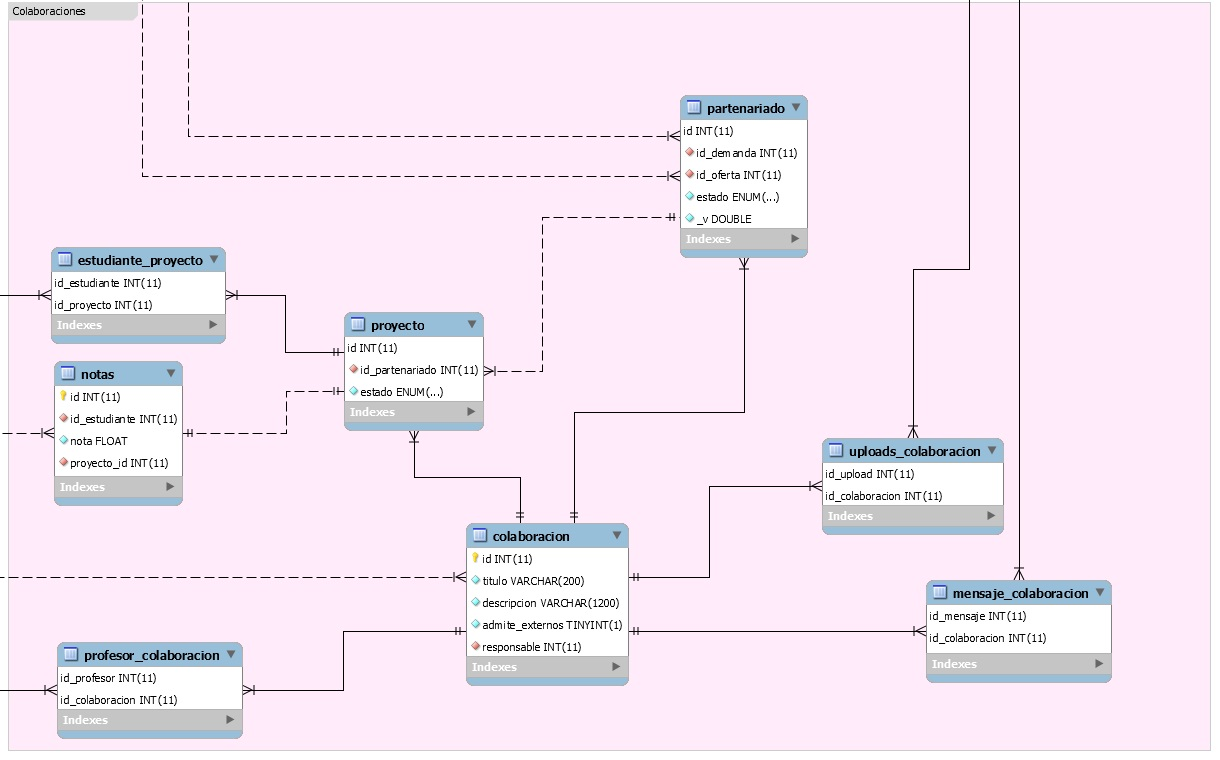
\includegraphics[width=\textwidth]{colaboracion}
\begin{itemize}
	\item DAOColaboracion: se encarga de manejar toda la información relacionada con los proyectos y los partenariados, desde sus participantes, ya sean profesores o alumnos hasta los mensajes y archivos asociados a estos proyectos o partenariados. Este DAO se llama así porque tiene con piedra angular la clase 			Colaboración.
	Esta clase fue creada para hacer de padre de las clases partenariado y proyecto y así evitar la repetición de métodos y atributos similares. Utiliza los transfer TColaboracion, TPartenariado y TProyecto.

	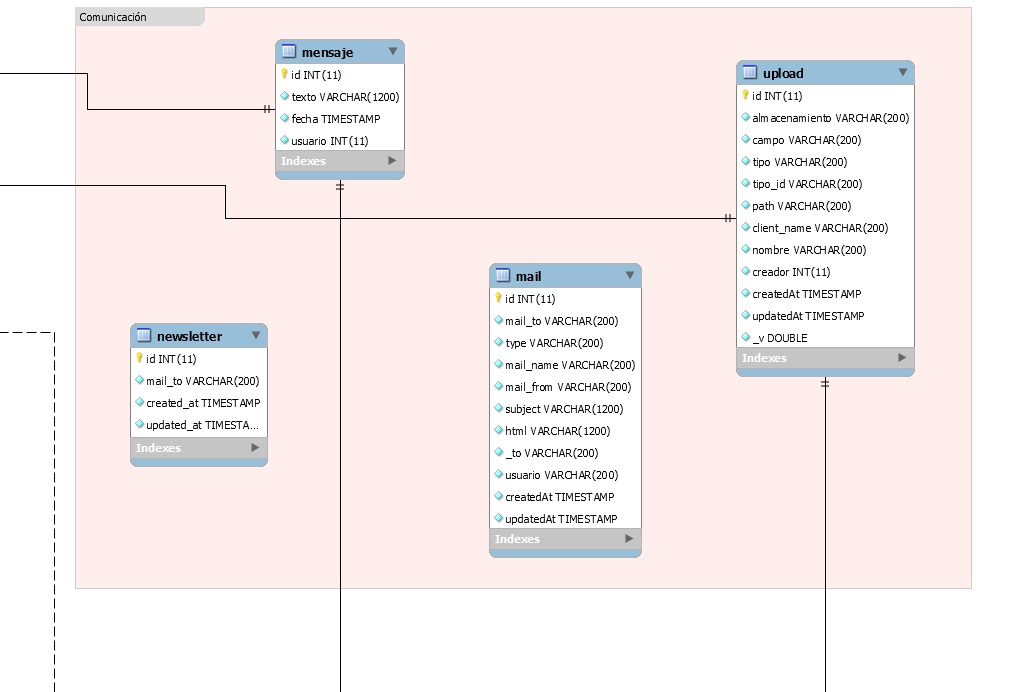
\includegraphics[width=\textwidth]{comunicacion}
	\item DAOComunicacion: se encarga de manejar toda la información relacionada con todas las formas de comunicación disponibles, desde los mensajes y los uploads que se pueden intercambiar durante las distintas fases de un partenariado o proyecto hasta los emails o las newsletter a las que se pueden suscribir los 		usuarios. Por lo tanto utiliza los transfer TUpload, TMensajes, TMail y TNewsletter

	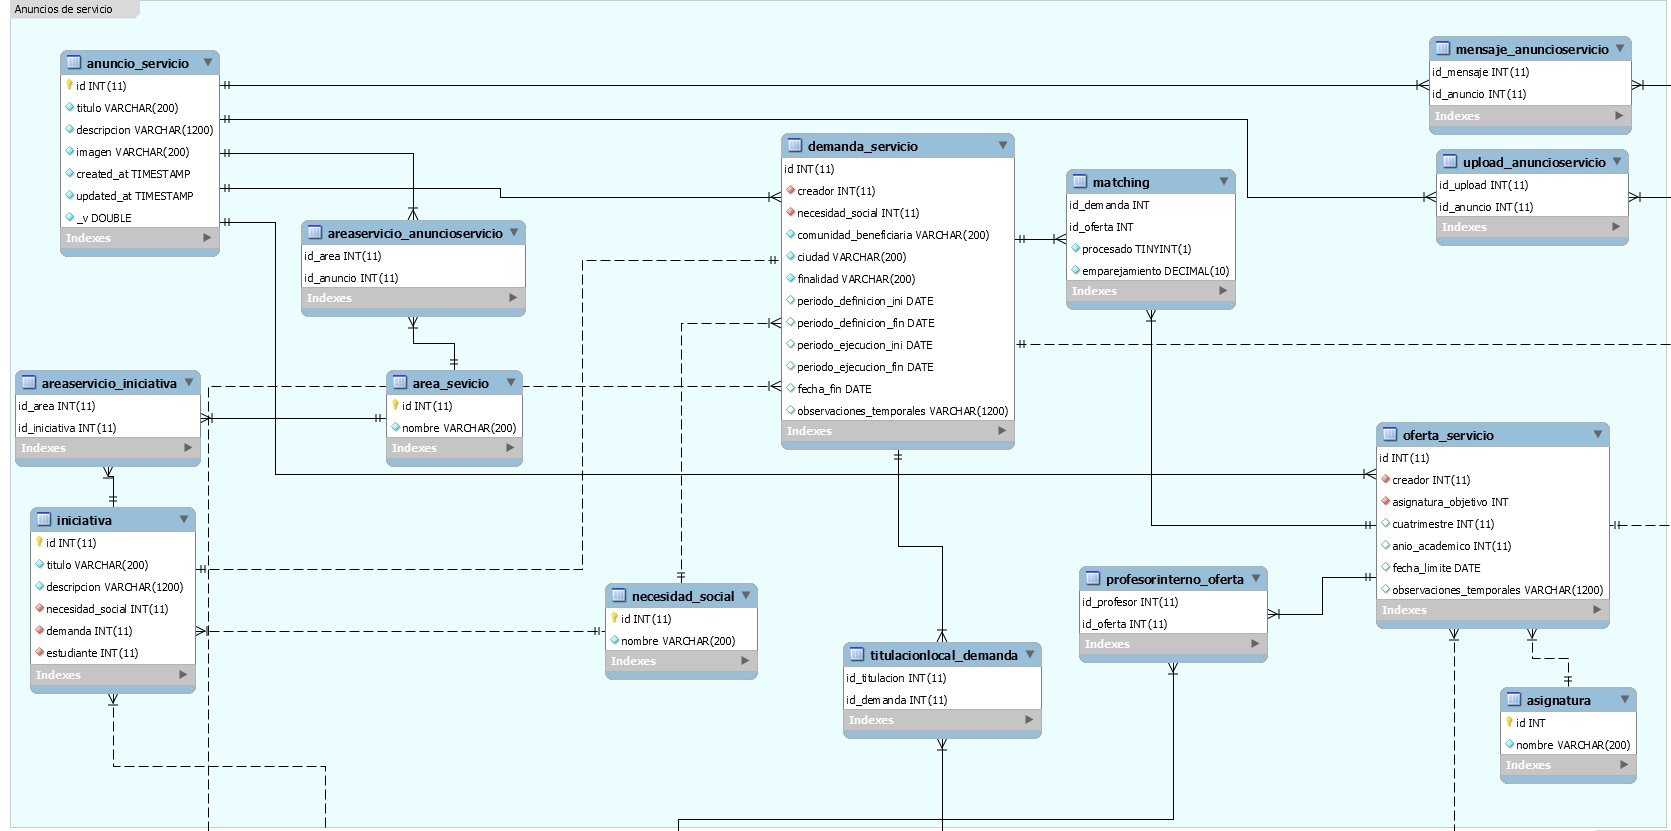
\includegraphics[width=\textwidth]{anuncio}
	\item DAOTentativa: trata toda la información relacionada con ofertas y demandas y sus relaciones con la titulación local ofrecida por la universidad, las áreas de servicio y las necesidades sociales que pudiera tener la demanda. 
	Al igual que antes se creó una clase padre llamada anuncio para evitar la repetición de atributos en las clases oferta y demanda y en sus derivadas. Este DAO también se encarga de las iniciativas, que son propuestas de proyecto realizadas por un alumno a la espera de que se le dé el visto bueno, y de los mensajes y 		uploads que pudieran tener tanto la oferta como la demanda. Para poder llevar a cabo esta función, utiliza los transfer TIniciativa, TOfertaServicio, TAnuncioServicio y TDemandaServicio.

	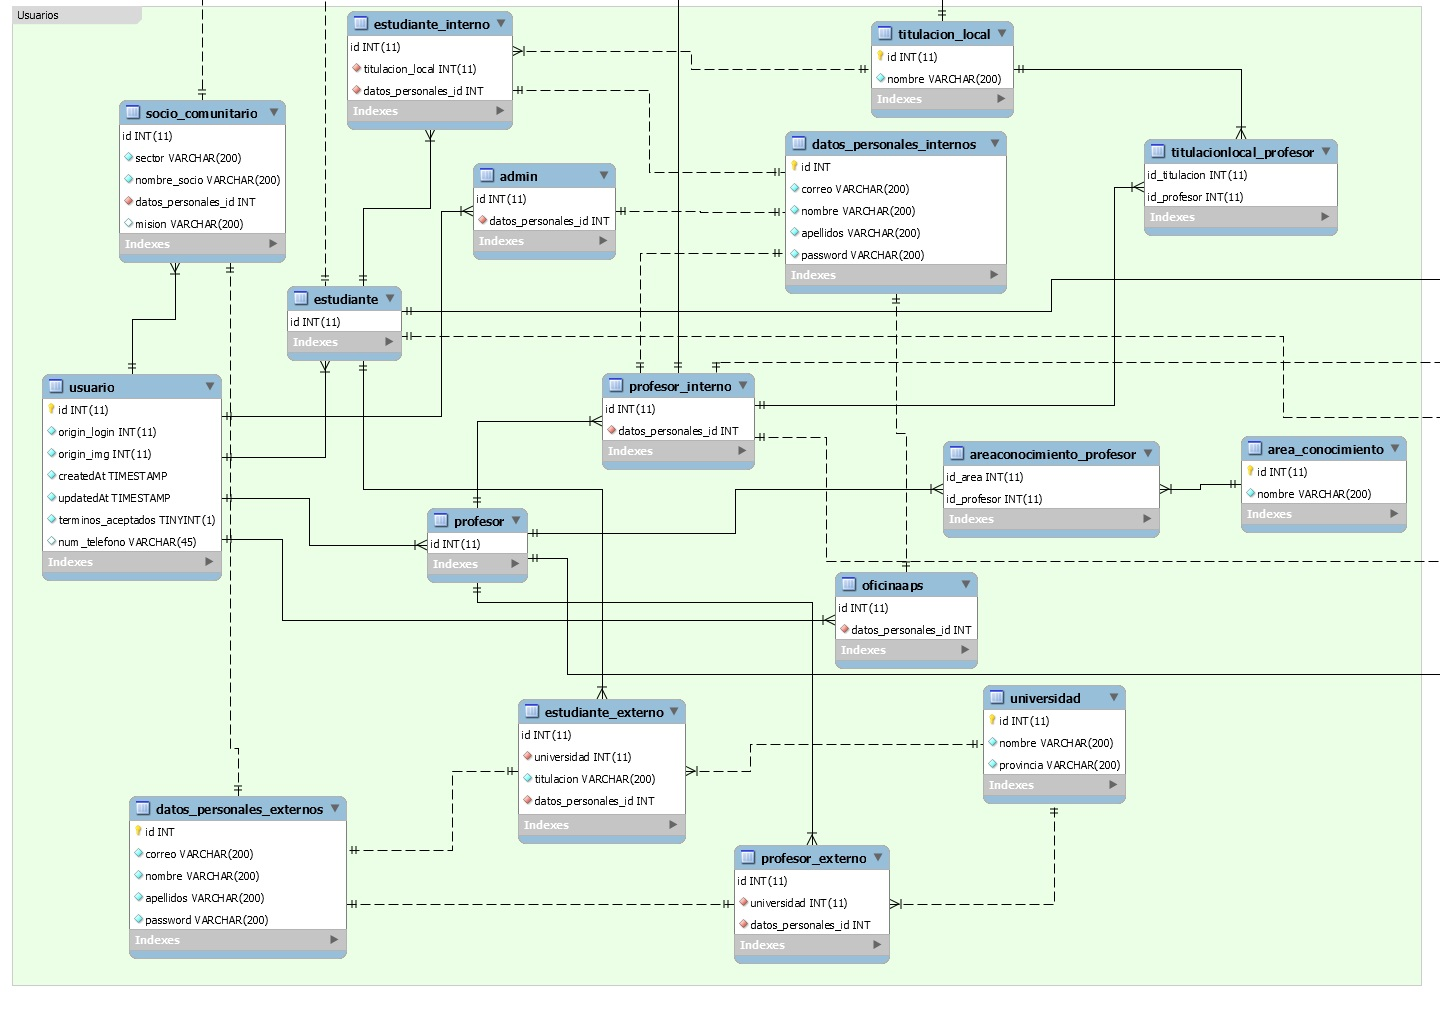
\includegraphics[width=\textwidth]{usuarios}
	\item DAOUsuario: se encarga de manejar los datos pertenecientes a las distintas clases de usuario, que son: profesor interno, profesor externo, estudiante interno, estudiante externo, admin, entidad y oficina APS.
	Además de estas clases también interactúa con los respectivos padres de cada una de ellas y con las titulaciones locales, áreas de conocimiento y universidades que son necesarias para completar los atributos de los profesores.
	Para ello utiliza los transfer TAdmin, TEntidad, TUsuario, TProfesor, TOficinaAPS, TEstudiante, TProfesorExterno, TProfesorInterno, TEstudianteInterno y TEstudianteExterno

	
	\end{itemize}
	Se ha intentado que los DAO tengan todas las funcionalidades necesarias para que la aplicación pudiera seguir funcionando tras sufrir cambios sin necesidad de actualizar los DAO con frecuencia, pero resulta imposible saber qué nuevas funcionalidades puede adquirir la aplicación o que cambios podría sufrir el modelo 		de datos así que aunque cuenta con bastantes funcionalidades será necesario actualizarlo sobre la marcha si en un futuro la aplicación sufre cambios





\end{document}
